%%=================== Compiler Directives =================%%
%%                                                         %%
% !TeX program = pdflatex								    	
% !TeX encoding = utf8
% !BIB TS-program =bibtex8
%%                                                         %%
%%=========================================================%%



%%==================================================================================%%
%%                                                                                  %%
%%  сайт конференції conf.ipt.kpi.ua				                                %%
%%  проект на ShareLaTeX https://ru.sharelatex.com/project/56e308d7bad2a71c56327601 %%
%%  проект на OverLeaf https://www.overleaf.com/read/ckvrdbwwkzng                   %%
%%                                                                                  %%
%%==================================================================================%%



%%===================== Class Options =====================%%
%%                                                         %%
%%                                                         %%
				\documentclass{ConfFTI}					
%%                                                         %%		
%%   incollection  - create black footers and headers 	   %%
%%   alone 		   - create pagenumber in footers          %%
%%=========================================================%%



%%===================== Package Placing ===================%%

\usepackage[most]{tcolorbox}
\usepackage{makecell}
\usepackage{booktabs}
\usepackage{tabularx}
\usepackage{mathtools}
\usepackage{dsfont}
\usepackage{mathrsfs}
\usepackage{wrapfig}
\usepackage{graphicx}
%usepackage{xurl}

%==== Пакет для створення діаграм та графіків =====
\usepackage{forest}
\usepackage{tikz}
\usepackage{pgfplots}
\usetikzlibrary{shadows,arrows.meta}

%%================== Команди користувача ==================%%
%%            Тут можна визначити власні команди           %%
\def\templateurl{%
\href{https://drive.google.com/file/d/1YrrTXnwaIcydBJLFS5BM6uj-yosnkRl3/view}%
{\texttt{\jobname.zip}}}
\DeclareMathOperator*{\argmax}{arg\,max}
\DeclareMathOperator*{\argmin}{arg\,min}
\graphicspath{ {./images/} }
%%=========================================================%%




%%======================= Назва тез =======================%%
%%                                                         %%
%%                                                         %%
\title{Задача стерео-зору в умовах поступового надходження даних }
%%                                                         %%		
%%                                                         %%
%%=========================================================%%



%%======================== AUTHORS ========================%%
%%  Якщо бажаєте, введіть e-mail автора в квадратних дужках:	
\author[\email]{Кириленко~І.~А.}{1} % Команда \email -- вставляє значення наведене в реєстраційній формі					    					

%\author{~Кригін~В.~М.}{1, 2}

%\author{А.~В.~Третій}{2}

%% Якщо  автор працює в кількох установах, то треба вводити номери установ через кому, наприклад так:
%\author[email3@mail.com]{А.~В.~Четвертий}{1,2}

%% значки "~" біля ініціалів і прізвищ означають нерозривний пробіл.



%%========= Назви установ, в яких працюють автори ==========%%

\affiliation{\ntuuipt}{1}
%% Тут введіть установув якій працює, або навчається перший автор.
%% Введіть \ntuu якщо автор навчається, або працює в НТУУ "КПІ"
%% Введіть \ntuuipt якщо автор навчається, або працює в Фізико-технічному інституті
%\affiliation{Міжнародний науково-навчальний центр інформаційних технологій та систем НАН України та МОН України}{2}
%% Тут введіть установу в якій працює, або навчається другий автор



%%================== Реєстраційна форма ===================%%
%%                                                         %%
%%                                                         %%
\FullName{Кириленко Іван Андрійович}                            %% Повне ім'я доповідача (перший автор)
\Birthday{17.07.1999}                                      %% Дата народження доповідача
\Position{студент}                                         %% Посада доповідача
\phone{+380992036799}                                      %% Телефонний номер доповідача
\authoremail{mr\_thor@gmail.com}                           %% Email доповідача 
\confsection{Математичнi методи комп’ютерного моделювання та кiбернетичної безпеки}                   %% Секція конференції, на яку подається доповідь
\copynum{0}                                                %% Кількість копій збірника матеріалів, необхідних автору 0/1/2 тощо
\NeedLiving{ні}                                            %% Потреба в житлі (Ні/Хостел/Готель/інше)
\NeedInvitation{так}                                        %% Чи потрібне запрошення на конференцію?
%%                                                         %%		
%%                                                         %%
%%=========================================================%%



%%============ Тут вводьте номери PACS або УДК ============%%
%%                                                         %%
%\pacs{ }
\udc{501}
%%                                                         %%
%%=========================================================%%



%%============= Тут заповніть ключові слова ===============%%
\keywords{комп'ютерний зір, стерео-зір, динамічне програмування}
\abstract{
	 %Дана робота розглядає задачу стереозору в умовах різних типів надходження даних та пропонує методи, які для цих випадків, є більш ефективними, ніж класичні.
	 }



%%====================================================================================%%
\begin{document}


	
%%=========Замість слова ukrainian (russian, english) введіть мову ваших тез =========%%
%%                                                                                    %%	
\PaperLanguage{ukrainian} %
%%                                                                                    %%
%%====================================================================================%%


%%====================================================================================%%
\section*{Вступ}
%%====================================================================================%%
%Задача отримання інформації про глибину зображення та відстані до об'єктів на ньому -- одна з основних задач у сфері комп'ютерного зору.  
%Немає нічого несподіваного в тому, що основний спосіб сприйнятя навколишньго світу людиною знайшов знайшов місце у різних галузях.
%для більшої ефективності під кожну окрему задачу алгоритми варто модифікувати окремо.
	Від автономної навігації \cite{stereoNav} та фотограмметрії cite{stereoPG} до доповненої реальності cite{stereoAR} -- задачі стерео-зору мають багато застосувань. Задача стерео-зору полягає у використанні двох або більше камер для отримання даних про відстань до об'єктів cite{stereoReview}. Ідея методу полягає в порівняні зображень об'єкта отриманих під різними кутами та пошуку скалярного поля зсувів (або карти зсувів -- від англ. disparity map).
	
В цій роботі розглядаються одновимірні алгоритми пошуку карти зсувів. Це означає, що кожен рядок зображення ми опрацьовуємо незалежно від інших. Такий підхід вимагає попередньої ректифікації зображення, проте є більш швидким та дає непогані результати (рис. \ref{results}).
%results
\begin{figure}[h!]
	\centering
	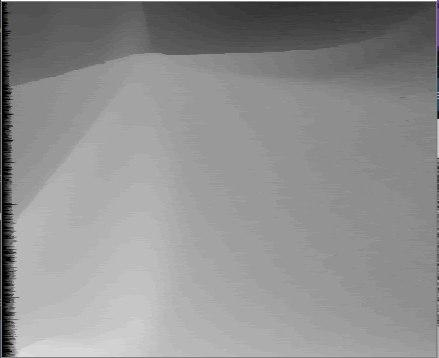
\includegraphics[scale = 0.3]{result}
	%$ results.png $
	\caption{Результат роботи одновимірного алгоритму}
	\label{results}
\end{figure}

Далі під <<зображенням>> будемо розуміти деякий рядок вихідного зображення.
Перший розділ присвячено постановці задачі стерео-зору та методам її вирішення в умовах повних даних. У другому розділі розглянуто модифікації цих методів для випадку поступового надходження даних.


%%====================================================================================%%
\section{Пошук зсувів при повних даних} \label{sec1}
%%====================================================================================%%

%%====================================================================================%%	
\subsection{Постановка задачі} 
%%====================================================================================%%
	Нехай $ n $ -- довжина зображення, а $I = \{1, 2, .., n\}$ -- множина координат пікселів. Ліве і праве зображення задамо як функції $ \mathcal{L} : I \rightarrow R $ та $ \mathcal{R} : I \rightarrow R $. Тобто $\mathcal{L}(i)$ -- інтенсивність $i$-го пікселя на лівому зображені, а $\mathcal{R}(i)$ -- інтенсивність $i$-го пікселя на правому зображені. Така постановка природно узагальнюється на випадок кольорових зображень. Також введемо множину зсувів $D = \{0, ... , D_{max}\}$, де $D_{max}$ -- значення максимального зсуву, та підбирається експериментально.

Для вирішення задачі нам потрібно кожному пікселю лівого зображення знайти відповідний йому піксель на правому зображенні (\ref{mapping}). Тобто для кожного пікселя з номером $i$ лівого зображення знайти таке $ d_i \in D$, щоб піксель правого зображення  з номером $i - d_i$ -- відповідав йому.
%mapping
\begin{figure}[h!]
	\centering
	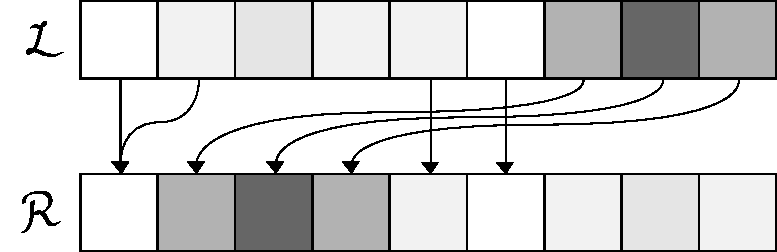
\includegraphics[scale = 0.5]{mapping.pdf}
	\caption{Пошук відповідних пікселів}
	\label{mapping}
\end{figure}

Проте, не будь яка пара пікселей може знаходитися у відповідності -- пікселю з номером $i$ на лівому зображені можуть відповідати тільки ті пікселі  правого зображення з номером $j$, для яких $i \leq j$. Переконатися в цьому можна тримаючи перед собою олівець та по черзі закриваючи то праве, то ліве око. Для правого ока олівець буде знаходитися лівіше ніж для лівого

Тож треба знайти таку послідовність $\overline{d} \in {D}^n$, яка б мінімізувала штрафну функцію
\begin{equation}
\omega(\overline{d}) = \sum\limits_{i = 1}^n h(i, d_i) + \sum\limits_{i = 1}^{n-1} g(d_i, d_{i + 1}),
\label{penalty}
\end{equation}
$$ h(i, d_i) = | \, \mathcal{L} (i) - \mathcal{R} (i - d_i) \, |, $$ 
$$ g(d_i, d_{i+1}) = \alpha \, | \; d_i - d_{i+1}\; |. $$

Де $ h(i, d_i) $ відповідає за схожість кольору пікселів, $ g(d_i, d_{i+1}) $ -- за гладкість поля зсувів, а $ \alpha $ -- коефіцієнт згладжування.


%%====================================================================================%%	
\subsection{Зведення задачі до пошуку найкоротшого  шляху на графі}\label{G_definition}
%%====================================================================================%%
Представимо задачу пошуку послідовності $ \overline{d} $ , що мінімізує штрафну функцію (\ref{penalty}), як пошук найкоротшого шляху через орієнтований зважений граф $G = <\mathcal{V}, \mathcal{E}>$ (\ref{graphG}). Множина вершин якого
$$ \mathcal{V} = \{ \sigma(i, d) \, | \, i \in I, \, d \in D \} \cup \{ S, E \}.$$ Вершина $\sigma(i, d)$ має вагу $h(i, d) \;, \; i \in I, \, d \in D .$\\
Множина ребер
\begin{align*}
\mathcal{E} = &\bigcup\limits_{d \in D }<S, \sigma(1, d) > \; \cup 
\\ \cup &\bigcup\limits_{\substack{d \in D}} <\sigma(n, d), E > \; \cup 
\\ \cup &\bigcup\limits_{\substack{i = 1..n-1 \\d \in D \\d' \in D}} <\sigma(i, d), \sigma(i+1, d') >.
\end{align*}
Ваги ребер
\begin{itemize}
\item З $ S $ в $ \sigma(1, d) $ -- $ 0 $, $ d \in D $
\item З $ \sigma(n, d) $ в $ E $ -- $ 0 $, $ d \in D $
\item З $ \sigma(i, d) $ в $\sigma(i + 1, d ') $ -- $ g(d, d') $, $ \; d, d' \in D, i \in I $
\end{itemize}

\begin{figure}[h!]
	\centering
	\tikzset{>=latex}
	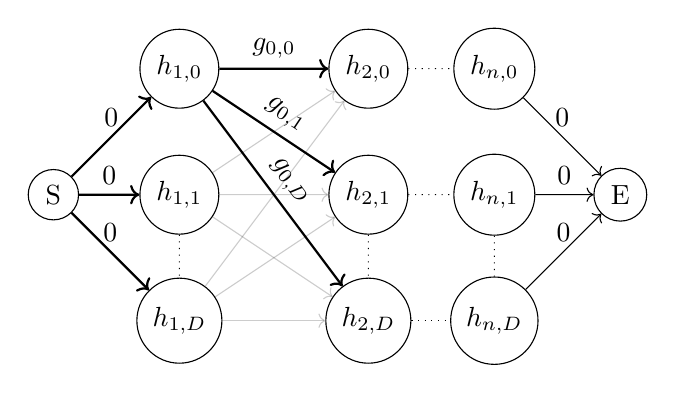
\begin{tikzpicture}[scale=0.8]
	\tikzstyle{vertex} = [circle, draw=black]
	\tikzstyle{edge} = [->, thick]

%----------Виходить такий граф:------------------------------
	\node[vertex] (s) at (0,2) {S};
	
	\node[vertex] (v1n) at (2,0) {$h_{1,D}$};
	\node[vertex] (v11) at (2,2) {$h_{1,1}$};
	\node[vertex] (v10) at (2,4) {$h_{1,0}$};
	
	\path[->, thick] (s) edge node[ above ] {0} (v1n);
	\path[->, thick] (s) edge node[ above ] {0} (v11);
	\path[->, thick] (s) edge node[ above ] {0} (v10);
	
	\draw[dash pattern=on \pgflinewidth off 2pt] (v11)--(v1n);
	
%------------------------------------------------------------
	\node[vertex] (v2n) at (5,0) {$h_{2,D}$};
	\node[vertex] (v21) at (5,2) {$h_{2,1}$};
	\node[vertex] (v20) at (5,4) {$h_{2,0}$};

	\path[->, opacity=0.2] (v11) edge node[ above,sloped ] {} (v2n);
	\path[->, opacity=0.2] (v11) edge node[ above,sloped ] {} (v21);
	\path[->, opacity=0.2] (v11) edge node[ above,sloped ] {} (v20);
	
	\path[->, opacity=0.2] (v1n) edge node[ above,sloped ] {} (v2n);
	\path[->, opacity=0.2] (v1n) edge node[ above,sloped ] {} (v21);
	\path[->, opacity=0.2] (v1n) edge node[ above,sloped ] {} (v20);
	
	%Selected
	\path[->, thick] (v10) edge node[ above,sloped ] {$g_{0,D}$} (v2n);
	\path[->, thick] (v10) edge node[ above,sloped ] {$g_{0,1}$} (v21);
	\path[->, thick] (v10) edge node[ above,sloped ] {$g_{0,0}$} (v20);
	
	\draw[dash pattern=on \pgflinewidth off 2pt] (v21)--(v2n);
	
	
%------------------------------------------------------------
	\node[vertex] (vnn) at (7,0) {$h_{n,D}$};
	\node[vertex] (vn1) at (7,2) {$h_{n,1}$};
	\node[vertex] (vn0) at (7,4) {$h_{n,0}$};


	\draw[dash pattern=on \pgflinewidth off 2pt] (v2n)--(vnn);
	\draw[dash pattern=on \pgflinewidth off 2pt] (v21)--(vn1);
	\draw[dash pattern=on \pgflinewidth off 2pt] (v20)--(vn0);
	
	\draw[dash pattern=on \pgflinewidth off 2pt] (vn1)--(vnn);
%------------------------------------------------------------
	\node[vertex] (e) at (9,2) {E};

	\path[->] (vnn) edge node[ above ] {0} (e);
	\path[->] (vn1) edge node[ above ] {0} (e);
	\path[->] (vn0) edge node[ above ] {0} (e);
	
	\end{tikzpicture}
	\caption{Граф $G$}
	\label{graphG}
\end{figure}


Тоді послідовність $\overline{d}$ -- послідовність вершин через які проходить найкоротший шлях з $S$ в $E$, і буде мінімізувати штрафну функцію $ \omega(\overline{d}) $ (\ref{penalty}).

Позначимо довжину найкоротшого шляху з вершини S в вершину $ \sigma(i, d) $ як $ f_i (d) $. Тоді $ \forall d \in D $ 
\begin{align*}
f_1 (d) &= h(1, d), \\
f_2 (d) &=  \min\limits_{d' \in D}\Big( f_1(d) + g(d', d) \Big) + h(2, d), \\
&\vdots \\
f_i (d) &= \min\limits_{d' \in D}\Big( f_{i-1}(d) + g(d', d) \Big) + h(i, d).
\end{align*}
Тоді елементи послідовності $\overline{d}$ знаходимо за формулами:
\begin{align*}
d_n &= \argmin\limits_{d' \in D}{\big( f_n(d') \big)}, \\
d_i &= \argmin\limits_{d' \in D}{\big( f_{i}(d') + g(d',d_{i+1})\big) \; i = \overline{n-1, 1}}
\end{align*}
%%====================================================================================%%
\section{Пошук зсувів при поступово надходжуючих даних}
%%====================================================================================%%

Метод описаний в частині \ref{sec1} потребує наявності всіх даних до початку обчислень. В ситуації, коли дані надходять повільно, цей метод не є самим ефективними. Доводиться чекати надходження всіх даних і тільки потім починати обчислення, адже ми не можемо розрахувати ваги деяких вершин.
Замість цього можна проводити деякі розрахунки над частиною даних, яка вже надійшла, цим самим зменшивши час роботи алгоритму після отримання всіх даних.

%====================================================================================
\subsection{Випадок 1 -- дані надходять по порядку} \label{2.1}
%================================================================================

Нехай на початку нам невідомі жодні пікселі (рис. \ref{2.1nodata}), тож ми не можемо обчислити вагу жодної з вершин графа $G$ (\ref{G_definition}).  
%2.1nodata
\begin{figure}[h!]
	\centering
	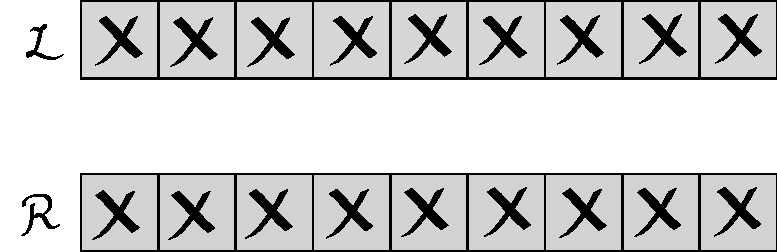
\includegraphics[scale = 0.5]{allclosed2.pdf}
	\caption{Немає даних}
	\label{2.1nodata}
\end{figure}

\label {2.1-style} Будемо називати вершину <<закритою>> якщо ми не можемо обчислити вагу вершини, а якщо можемо -- назвемо її <<відкритою>>. 
Тож на початку всі вершин графу $G$ закриті.

Нехай тепер нам поступово, по порядку надходить по одному пікселю кожного зображення. Коли нам відомий лише перший піксель кожного зображення (рис.\ref{2.2onedata})
%2.2onedata
\begin{figure}[h]
	\centering
	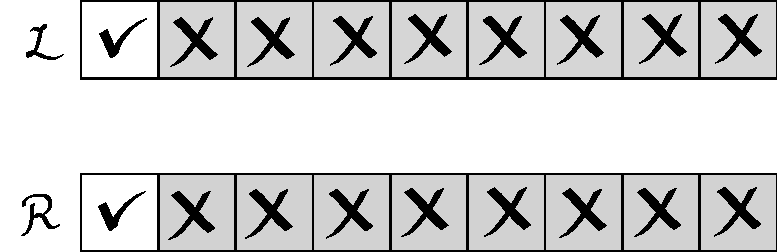
\includegraphics[scale = 0.5]{onestereoknown.pdf}
	\caption{Відомі перші пікселі обох зображень}
	\label{2.2onedata}
\end{figure}
то граф $G$ матиме лише одну відкриту вершину $\sigma(1, 0)$. Коли нам буде відомо два перші пікселі, то нам стануть відомі ще й вершини 
$\sigma(1, 1)$ та $\sigma(2, 0)$. Таким чином, при надходженні перших $k$ пікселів обох зображень, в графі $G$ будуть відкриті вершини 
$\sigma(i, d_i)$, де $i \in I, i \leq k$, a $d_i \in D, 0 \leq d_i \leq \min{\big( k - i, D_{max}  \big)}$. І тільки коли $k$ буде більше за $D_{max}$, всі вершини в першому стовпчику $\sigma(1, d) \; \forall d \in D $ будуть відкритими, і ми зможемо починати оптимізацію:

Нехай $G^0 = <\mathcal{V}^0, \mathcal{E}^0> = <\mathcal{V}, \mathcal{E}> = G $. Нехай також $s^0(d) = 0, \; \forall d \in D $. Для відновлення послідовності 
$\overline{d}$ введемо матрицю $\hat{\mathcal{P}}$ розмірності $n \times (D_{max} + 1)$.  $$p_{1,d} = 0, \forall d \in D. $$

Як тільки перші $D_{max} + t, \; ( 1 \leq t < n - D_{max})$ стерео-пікселей стають нам відомі, шукаємо граф $G^t$:
\begin{enumerate}
	\item 
		$\forall d \in D :$\\
		$s^t(d) = \min\limits_{d' \in D} \big( s^{(t-1)}(d') + h(t, d') + g(d', d) \big).$\\
		$p_{t+1,d} = \argmin\limits_{d' \in D}{\big( s^t(d) \big) }$.
	\item 
		$\mathcal{V}^t = \mathcal{V}^{t-1} \setminus \{ \sigma(t, d) \; | \; d \in D \}.$
	\item %\begin{align*}
		$\mathcal{E}^t = \mathcal{E}^{t-1} \setminus$\\
		$\setminus \bigcup\limits_{d \in D} <S, \sigma(t, d) > \setminus $\\
		$\setminus \bigcup\limits_{\substack{d \ in D \\ d' \in D}} <\sigma(t, d), \sigma(t+1, d') > \cup $\\
		$\cup \bigcup\limits_{d \in D} <S, \sigma(t+1, d) >.$\\
		А вага ребра $ <S, \sigma(t+1, d) >$ -- $ s^t(d)$ %, \; \forall d \in D$.
		%\end{align*}
	\item 
		$G^t = <\mathcal{V}^t, \mathcal{E}^t> $ 
\end{enumerate}



Кожен новий граф $G^t$ матиме на $(D_{max})^2$ менше ребер, ніж граф $G^{t-1}$. Таким чином, на момент приходу останніх пікселів, нам треба буде опрацювати лише $D_{max}$ ребер. А якщо б ми спочатку чекали приходу всіх даних, а тільки потім починали обчислення, нам треба було опрацювати 
$(n-1)(D_{max})^2$ ребер.

Коли ж нам стануть відомі всі $n$ пікселей обох зображень, нам залишиться тільки знайти
$$ d_n = \argmin\limits_{d' \in D} \big( s^{(n-D_{max}-1)}(d') + h(n, d') \big),$$
та відновити послідовність $\overline{d}$ через матрицю $\hat{\mathcal{P}}$ --
$$ d_i = p_{i+1,d_{i+1}}, i = \overline{n-1, 1}. $$


%$G^0 = <\mathcal{V}^0, \mathcal{E}^0>

%Як тільки нам буде відомо перші $D_{max} + 1$ пікселей на обох зображеннях -- всі вершини $\sigma(1, d), \; \forall d \in D$ стануть відкритими. Отже можемо знайти довжини найкоротших шляхів з початкової вершини $S$ до кожної з вершин у другому стовпчику (\ref{Goptstart}). 

%І як тільки ми їх знайдемо, тоді всі інші можливі шляхи з $S$ до $ \sigma(2,d), \, d \in D$ нам не потрібні. Тому ми відкидаємо всі вершини в першому стовпчику, і вводимо ребра $<S, \sigma(2, d) >, \, d \in D$ (рис.\ref{Goptafter}), з вагою $${g_d}^{(1)} = \min\limits_{k=0}^{D_{max}} (h_{k} + g_{kd}).$$ 
	
%Цим самим зменшуємо кількість ребер на $(D_{max})^2$. При надходженні наступних пікселей повторюємо цю операцію, але ваги нових ребер $g_d^{(i)}$ вже будуть враховувати попередні оптимізації --
%$${g_d}^{(i)} = \min\limits_{k=0}^{D_{max}} ({g_k}^{(i-1)} + h_{k} + g_{kd}).$$ 

%Після кожної такої оптимізації кількість ребер в графі зменшується на $(D_{max})^2$. Таким чином, коли нам будуть відомі всі пікселі обох зображень, нам зали
%Після отримання перших $D_{max} + 1$ пікселів обох зображень при кожному наступному відкритому пікселі зменшуємо кількість ребер на $(D_{max})^2$. Такий метод ефективний, коли довжина зображення $n$ більша за $D_{max}$.	
 
%%====================================================================================%%

\subsection{Випадок 2 -- повністю відоме одне з зображень} \label{2.2}
%%====================================================================================%%
Нехай на початку нам відоме лише ліве зображення (рис. \ref{2.2oneimage}), у такому разі ми теж не можемо обчислити вагу жодної з вершин графа $G$. Будемо використовувати ті ж позначення як і в  \ref{2.1-style}. Тоді граф $G$ буде мати вигляд як і на (рис. \ref{2.1nodata}).
%allclosed
\begin{figure}[h!]
	\centering
	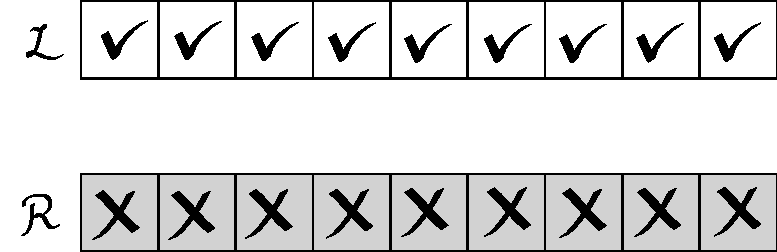
\includegraphics[scale = 0.5]{allclosed.pdf}
	\caption{Відомо лише одне з зображень}
	\label{2.2oneimage}
\end{figure}

Нехай тепер нам стає відомий якийсь  один (наприклад другий) піксель правого зображення (рис. \ref{2.2oneRpixel}). 
\begin{figure}[h!]
	\centering
	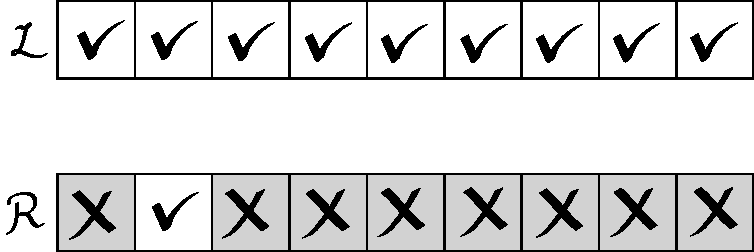
\includegraphics[scale = 0.5]{pixelknown.pdf}
	\caption{Відомий другий піксель правого зображення}
	\label{2.2oneRpixel}
\end{figure}
	
Тоді у графі $G$ одразу всі вершин у другому стовпчику стануть відкритими ().
\begin{figure}[h!]
	\centering
	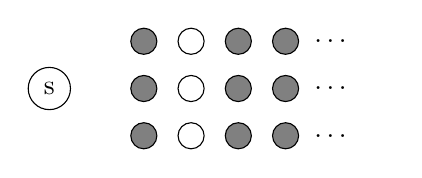
\begin{tikzpicture}[scale=0.6]
	\tikzstyle{vertex_closed_1} = [circle, draw=black, fill=gray, opacity=0.3]
	\tikzstyle{vertex_closed_2} = [circle, draw=black, fill=gray]
	\tikzstyle{vertex_opened} = [circle, draw=black]

%------------------------------------------------------------
	\node[vertex_opened] (s) at (-1,1) {s};

	\node[vertex_closed_2] (v00) at (1,0) {};
	\node[vertex_closed_2] (v01) at (1,1) {};
	\node[vertex_closed_2] (v02) at (1,2) {};
		
%------------------------------------------------------------
	
	\node[vertex_opened] (v10) at (2,0) {};
	\node[vertex_opened] (v11) at (2,1) {};
	\node[vertex_opened] (v12) at (2,2) {};
		
%------------------------------------------------------------
	
	\node[vertex_closed_2] (v20) at (3,0) {};
	\node[vertex_closed_2] (v21) at (3,1) {};
	\node[vertex_closed_2] (v22) at (3,2) {};
		
%------------------------------------------------------------
	
	\node[vertex_closed_2] (v30) at (4,0) {};
	\node[vertex_closed_2] (v31) at (4,1) {};
	\node[vertex_closed_2] (v32) at (4,2) {};
		
%------------------------------------------------------------

	\node[vertex_closed_2, opacity =0] (v40) at (6,0) {};
	\node[vertex_closed_2, opacity =0] (v41) at (6,1) {};
	\node[vertex_closed_2, opacity =0] (v42) at (6,2) {};
	
	\path (v30) -- node[auto=false]{\ldots} (v40);
	\path (v31) -- node[auto=false]{\ldots} (v41);
	\path (v32) -- node[auto=false]{\ldots} (v42);
	
	\end{tikzpicture}
	\captionof{figure}{граф $G$ при відсутності даних}
	\label{2.2G2col}
\end{figure}

При такій конфігурації можлива оптимізація. Припустимо, що найкоротший шлях проходить через вершини ${h^{(1)}}_{i}$ та ${h^{(3)}}_{j}$ (рис. \ref{2.2noopt}). Тоді ми точно знаємо що найкоротший шлях проходить через вершину ${h^{(2)}}_k$, де 
\begin{equation}\label{2.2k}
k = \argmin\limits_{l=0}^{D_{max}}{\big( g_{il} + {h^{(2)}}_l + g_{lj} \big) }
\end{equation}


%Simple graph 1
\begin{figure}[h!]
	\centering
	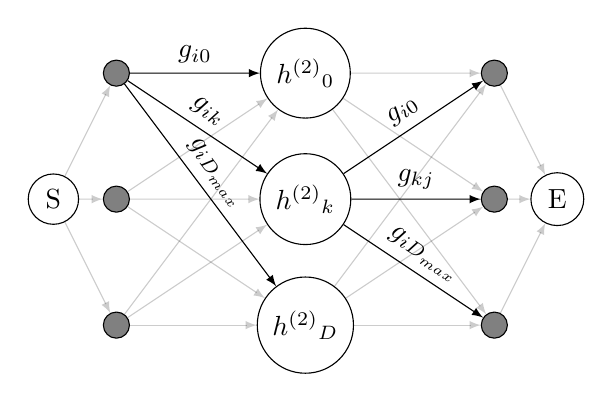
\begin{tikzpicture}[scale=0.8]
	
	\tikzstyle{vertex_closed} = [circle, draw=black, fill=gray]
	\tikzstyle{vertex_opened} = [circle, draw=black]
	%\tikzstyle{vertex} = [circle, draw=black]
	\tikzstyle{edge} = [->, thick]

%------------------------------------------------------------
	\node[vertex_opened] (s) at (0,2) {S};
	
	\node[vertex_closed] (v1n) at (1,0) {};
	\node[vertex_closed] (v11) at (1,2) {};
	\node[vertex_closed] (v10) at (1,4) {};
		
	\path[-latex, opacity=0.2] (s) edge node[ above ] {} (v1n);
	\path[-latex, opacity=0.2] (s) edge node[ above ] {} (v11);
	\path[-latex, opacity=0.2] (s) edge node[ above ] {} (v10);
%------------------------------------------------------------
	\node[vertex_opened] (v2n) at (4,0) {${h^{(2)}}_{D}$};
	\node[vertex_opened] (v21) at (4,2) {${h^{(2)}}_k$};
	\node[vertex_opened] (v20) at (4,4) {${h^{(2)}}_0$};
	
	\path[-latex, opacity=1] (v10) edge node[ above, sloped ] {$g_{iD_{max}}$} (v2n);
	\path[-latex, opacity=1] (v10) edge node[ above, sloped ] {$g_{ik}$} (v21);
	\path[-latex, opacity=1] (v10) edge node[ above, sloped ] {$g_{i0}$} (v20);
	
	\path[-latex, opacity=0.2] (v11) edge node[ above, sloped ] {} (v2n);
	\path[-latex, opacity=0.2] (v11) edge node[ above, sloped ] {} (v21);
	\path[-latex, opacity=0.2] (v11) edge node[ above, sloped ] {} (v20);
	
	\path[-latex, opacity=0.2] (v1n) edge node[ above, sloped ] {} (v2n);
	\path[-latex, opacity=0.2] (v1n) edge node[ above, sloped ] {} (v21);
	\path[-latex, opacity=0.2] (v1n) edge node[ above, sloped ] {} (v20);
%------------------------------------------------------------
	\node[vertex_closed] (v3n) at (7,0) {};
	\node[vertex_closed] (v31) at (7,2) {};
	\node[vertex_closed] (v30) at (7,4) {};

	\path[-latex, opacity=1] (v21) edge node[ above, sloped ] {$g_{iD_{max}}$} (v3n);
	\path[-latex, opacity=1] (v21) edge node[ above, sloped ] {$g_{kj}$} (v31);
	\path[-latex, opacity=1] (v21) edge node[ above, sloped ] {$g_{i0}$} (v30);
	
	\path[-latex, opacity=0.2] (v20) edge node[ above, sloped ] {} (v3n);
	\path[-latex, opacity=0.2] (v20) edge node[ above, sloped ] {} (v31);
	\path[-latex, opacity=0.2] (v20) edge node[ above, sloped ] {} (v30);
	
	\path[-latex, opacity=0.2] (v2n) edge node[ above, sloped ] {} (v3n);
	\path[-latex, opacity=0.2] (v2n) edge node[ above, sloped ] {} (v31);
	\path[-latex, opacity=0.2] (v2n) edge node[ above, sloped ] {} (v30);
%------------------------------------------------------------
	\node[vertex_opened] (e) at (8,2) {E};
	
	\path[-latex, opacity=0.2] (v3n) edge node[ above, sloped ] {} (e);
	\path[-latex, opacity=0.2] (v31) edge node[ above, sloped ] {} (e);
	\path[-latex, opacity=0.2] (v30) edge node[ above, sloped ] {} (e);

	\end{tikzpicture}
	\caption{Граф $G$ до оптимізації}
	\label{2.2noopt}
\end{figure}

Та на практиці ми ще не знаємо через які вершини проходить найкоротший шлях, тому проводимо цю операцію для кожної пари вершин $<{h^{(1)}}_i , {h^{(3)}}_j> \; \forall i,j \in D$. Для кожної вершини ${h^{(3)}}_{j}$ запам'ятовуємо вершину ${h^{(2)}}_{k}$, де $k$ визначається формулою (\ref{2.2k}). Після цього можемо замінити всі вершини у другому стовпчику та шляхи через них на ребра, що з'єднують вершину ${h^1}_i$ з ${h^3}_j \; \forall i,j \in D$ (рис. \ref{2.2opt}). Ваги цих ребер
$$g'_{ij} = \min\limits_{l=0}^{D_{max}} (g_{il} + h_{l} + g_{lj}) \; \forall i,j \in D.$$
%optimized graph 
\begin{figure}[h!]
	\centering
	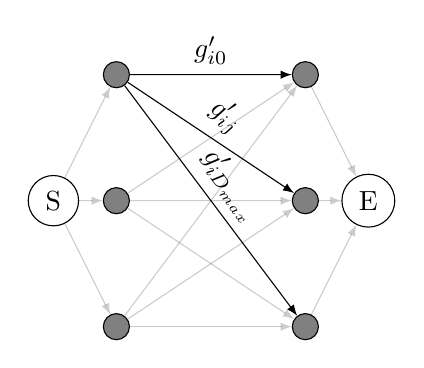
\begin{tikzpicture}[scale=0.8]

	\tikzstyle{vertex_closed} = [circle, draw=black, fill=gray]
	\tikzstyle{vertex_opened} = [circle, draw=black]
	%\tikzstyle{vertex} = [circle, draw=black]
	\tikzstyle{edge} = [->, thick]

%------------------------------------------------------------
	\node[vertex_opened] (s) at (0,2) {S};
	
	\node[vertex_closed] (v1n) at (1,0) {};
	\node[vertex_closed] (v11) at (1,2) {};
	\node[vertex_closed] (v10) at (1,4) {};
		
	\path[-latex, opacity=0.2] (s) edge node[ above ] {} (v1n);
	\path[-latex, opacity=0.2] (s) edge node[ above ] {} (v11);
	\path[-latex, opacity=0.2] (s) edge node[ above ] {} (v10);
	
%------------------------------------------------------------
	\node[vertex_closed] (v2n) at (4,0) {};
	\node[vertex_closed] (v21) at (4,2) {};
	\node[vertex_closed] (v20) at (4,4) {};
	
	\path[-latex, opacity=1] (v10) edge node[ above, sloped ] {$g'_{iD_{max}}$} (v2n);
	\path[-latex, opacity=1] (v10) edge node[ above, sloped ] {$g'_{ij}$} (v21);
	\path[-latex, opacity=1] (v10) edge node[ above, sloped ] {$g'_{i0}$} (v20);
	
	\path[-latex, opacity=0.2] (v11) edge node[ above, sloped ] {} (v2n);
	\path[-latex, opacity=0.2] (v11) edge node[ above, sloped ] {} (v21);
	\path[-latex, opacity=0.2] (v11) edge node[ above, sloped ] {} (v20);
	
	\path[-latex, opacity=0.2] (v1n) edge node[ above, sloped ] {} (v2n);
	\path[-latex, opacity=0.2] (v1n) edge node[ above, sloped ] {} (v21);
	\path[-latex, opacity=0.2] (v1n) edge node[ above, sloped ] {} (v20);

%------------------------------------------------------------
	\node[vertex_opened] (e) at (5,2) {E};
	
	\path[-latex, opacity=0.2] (v2n) edge node[ above, sloped ] {} (e);
	\path[-latex, opacity=0.2] (v21) edge node[ above, sloped ] {} (e);
	\path[-latex, opacity=0.2] (v20) edge node[ above, sloped ] {} (e);
	
	\end{tikzpicture}
	\caption{Граф $G$ після оптимізації}
	\label{2.2opt}
\end{figure}

При надходженні наступного пікселя з номером $m$ правого зображення, будемо проводити аналогічні операції: для кожної вершини ${h^{m+1}}_j$ запам'ятовувати , де 

Така оптимізація дозволяє нам зменшувати кількість ребер в графі на  $(\max{D})^2$ при кожному новому відкритому пікселі другого зображення. Таким чином, коли нам відкриється останній невідомий піксель, наш граф матиме лише $2 \max{D}$ ребер.

%%====================================================================================%%
\subsection{Випадок 3 -- дані надходять хаотично} 
%%====================================================================================%%

Нехай дані надходять у випадковому порядку.

\begin{center}
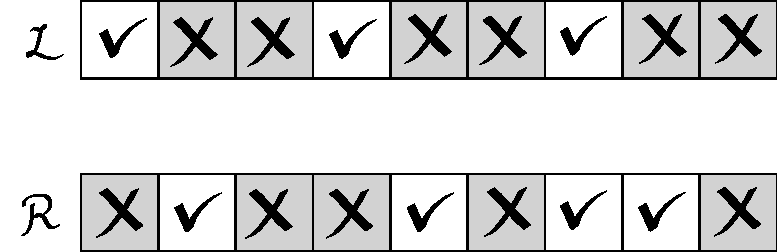
\includegraphics[scale = 0.5]{chaotic.pdf}
\end{center}
	
У такому випадку порядок відкриття вершин у графі нам невідомий. Припустмо що в нас відкрита одна вершина.
	
%Simple graph 2.1
\begin{center}
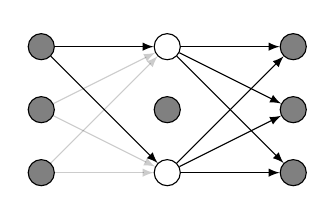
\begin{tikzpicture}[scale=0.8]

\tikzstyle{vertex_closed_1} = [circle, draw=black, fill=gray, opacity=0.3]
\tikzstyle{vertex_closed_2} = [circle, draw=black, fill=gray]
\tikzstyle{vertex_opened} = [circle, draw=black]
%\tikzstyle{vertex} = [circle, draw=black]
\tikzstyle{edge} = [->, thick]

%------------------------------------------------------------
	\node[vertex_closed_2] (v00) at (0,0) {};
	\node[vertex_closed_2] (v01) at (0,1) {};
	\node[vertex_closed_2] (v02) at (0,2) {};
		
%------------------------------------------------------------
	\node[vertex_opened]   (v10) at (2,0) {};
	\node[vertex_closed_2] (v11) at (2,1) {};
	\node[vertex_opened]   (v12) at (2,2) {};

	\path[-latex, opacity=1] (v02) edge node[above, sloped] {} (v12);
	\path[-latex, opacity=1] (v02) edge node[above, sloped] {} (v10);
	
	\path[-latex, opacity=0.2] (v01) edge node[above, sloped] {} (v12);
	\path[-latex, opacity=0.2] (v01) edge node[above, sloped] {} (v10);
	
	\path[-latex, opacity=0.2] (v00) edge node[above, sloped] {} (v12);
	\path[-latex, opacity=0.2] (v00) edge node[above, sloped] {} (v10);
	
%------------------------------------------------------------
	\node[vertex_closed_2] (v20) at (4,0) {};
	\node[vertex_closed_2] (v21) at (4,1) {};
	\node[vertex_closed_2] (v22) at (4,2) {};
	
	\path[-latex, opacity=1] (v12) edge node[above, sloped] {} (v20);
	\path[-latex, opacity=1] (v12) edge node[above, sloped] {} (v21);
	\path[-latex, opacity=1] (v12) edge node[above, sloped] {} (v22);
	
	\path[-latex, opacity=1] (v10) edge node[above, sloped] {} (v20);
	\path[-latex, opacity=1] (v10) edge node[above, sloped] {} (v21);
	\path[-latex, opacity=1] (v10) edge node[above, sloped] {} (v22);
	

\end{tikzpicture}
\captionof{figure}{До оптимізації}
\end{center}


%Simple graph 2.1
\begin{center}
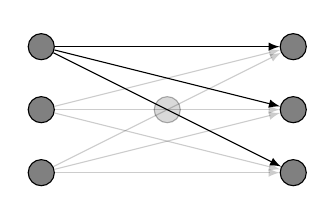
\begin{tikzpicture}[scale=0.8]

\tikzstyle{vertex_closed_1} = [circle, draw=black, fill=gray, opacity=0.3]
\tikzstyle{vertex_closed_2} = [circle, draw=black, fill=gray]
\tikzstyle{vertex_opened} = [circle, draw=black]
%\tikzstyle{vertex} = [circle, draw=black]
\tikzstyle{edge} = [->, thick]

%------------------------------------------------------------
	\node[vertex_closed_2] (v00) at (0,0) {};
	\node[vertex_closed_2] (v01) at (0,1) {};
	\node[vertex_closed_2] (v02) at (0,2) {};
		
%------------------------------------------------------------
	\node[vertex_closed_1] (v11) at (2,1) {};

	\node[vertex_closed_2] (v20) at (4,0) {};
	\node[vertex_closed_2] (v21) at (4,1) {};
	\node[vertex_closed_2] (v22) at (4,2) {};
	
%------------------------------------------------------------
	
	\path[-latex, opacity=1] (v02) edge node[above, sloped] {} (v22);
	\path[-latex, opacity=1] (v02) edge node[above, sloped] {} (v21);
	\path[-latex, opacity=1] (v02) edge node[above, sloped] {} (v20);
	
	\path[-latex, opacity=0.2] (v00) edge node[above, sloped] {} (v22);
	\path[-latex, opacity=0.2] (v00) edge node[above, sloped] {} (v21);
	\path[-latex, opacity=0.2] (v00) edge node[above, sloped] {} (v20);
	
	\path[-latex, opacity=0.2] (v01) edge node[above, sloped] {} (v22);
	\path[-latex, opacity=0.2] (v01) edge node[above, sloped] {} (v21);
	\path[-latex, opacity=0.2] (v01) edge node[above, sloped] {} (v20);

\end{tikzpicture}
\captionof{figure}{Після оптимізації}
\end{center}
%\path[-latex, opacity=0.2] (v11) edge[bend right=-20] node[] {} (v31);

Кількість ребер буде зменшуватися тільки тоді, коли відкрито більше половини вершин в стовпці.

 %%====================================================================================%%
\section{Приклади цитування літератури} %---ця секція для прикладу
%%====================================================================================%%
			
			
						
На кожне джерело має бути посилання в тексті тез.
Приклад оформлення посилань на підручник або книгу \cite{Vasylenko92}.
Якщо посилання йде на конкретну сторінку в книзі, то її слід вказувати таким чином \cite[стор. 4]{Vasylenko92}.
Якщо посилання йде книгу або монографію з кількома авторами, то посилання оформляються в такому вигляді
\cite{ObchTech93}. Якщо посилання на кілька джерел, то треба їх перераховувати через кому
\cite{Vasylenko92, ObchTech93}.
							
Посилання на статтю в журналі \cite{Ponomarenko86a, Malikov92}.
		
		
				
			
%%====================================================================================%%
\section*{Висновки}
%%====================================================================================%%
	
	
						
В цьому розділі узагальнюються головні підсумки обговорення результатів.
				
						
		
%%====================================================================================%%
%%                          Оформлення бібліографічних посилань                       %%
%%====================================================================================%%


		
%=== Якщо Вы НЕ плануєте скористатись власними бібліографічними файлами, закоментуйте два нижніх рядка ===%
		
\bibliographystyle{ugost2008} 																
\bibliography{\jobname} 														


			
%%=========================== Оформлення бібліографії ================================%%
% Якщо Ви НЕ плануєте користуватись власними бібліографічними файлами,
% розкоментуйте рядки знизу і заповніть відповідні поля
%%====================================================================================%%

		
%		
%	\begin{thebibliography}{1}
%	\def\selectlanguageifdefined#1{
%	\expandafter\ifx\csname date#1\endcsname\relax
%	\else\selectlanguage{#1}\fi}
%	\providecommand*{\href}[2]{{\small #2}}
%	\providecommand*{\url}[1]{{\small #1}}
%	\providecommand*{\BibUrl}[1]{\url{#1}}
%	\providecommand{\BibAnnote}[1]{}
%	\providecommand*{\BibEmph}[1]{#1}
%	\ProvideTextCommandDefault{\cyrdash}{\iflanguage{russian}{\hbox
%	  to.8em{--\hss--}}{\textemdash}}
%	\providecommand*{\BibDash}{\ifdim\lastskip>0pt\unskip\nobreak\hskip.2em plus
%	  0.1em\fi
%	\cyrdash\hskip.2em plus 0.1em\ignorespaces}
%	\renewcommand{\newblock}{\ignorespaces}
%	
%	\bibitem{Lvovsky}
%	\selectlanguageifdefined{russian}
%	\BibEmph{М.~Львовский~С.} Набор и верстка в
%	  системе \LaTeX. \BibDash
%	\newblock 3 {изд.} \BibDash
%	\newblock 2003. \BibDash
%	\newblock {С.}~448 c. \BibDash
%	\newblock {Режим доступа}:
%	  \BibUrl{http://www.mccme.ru/free-books/llang/newllang.pdf}.
%	
%	\bibitem{Voron05latex}
%	\selectlanguageifdefined{russian}
%	\BibEmph{В.~Воронцов~К.} \LaTeXe в примерах. \BibDash
%	\newblock 2005. \BibDash
%	\newblock {С.}~59 c. \BibDash
%	\newblock {Режим доступа}:
%	  \BibUrl{http://www.ccas.ru/voron/download/voron05latex.pdf}.
%	
%	\bibitem{Vasylenko92}
%	\selectlanguageifdefined{ukrainian}
%	\BibEmph{Василенко~М.~В.} Теорiя коливань:
%	  Навчальний посiбник. \BibDash
%	\newblock К.~: Вища школа, 1992.
%	
%	\bibitem{ObchTech93}
%	\selectlanguageifdefined{ukrainian}
%	Обчислювальна i прикладна математика:
%	  Зб.наук.пр. \BibDash
%	\newblock К.~: Либiдь, 1993.
%	
%	\bibitem{Ponomarenko86a}
%	\selectlanguageifdefined{russian}
%	\BibEmph{Пономаренко~Л.~А., Меликов~А.~З.}
%	  Ситуационное управление многоканальной
%	  системой с переменной структурой
%	  обслуживания неоднородного потока~//
%	  \BibEmph{Изв.\ АН Азерб.\ Респ. Сер.\ физ.-техн.\ и
%	  мат.\ наук}. \BibDash
%	\newblock 1986. \BibDash
%	\newblock Т.~7, {№}~6. \BibDash
%	\newblock {С.}~79--83.
%	
%	\bibitem{Malikov92}
%	\selectlanguageifdefined{russian}
%	\BibEmph{Меликов~А.~З., Пономаренко~Л.~А.}
%	  Оптимизация цифровой сети интегрального
%	  обслуживания с конечным числом
%	  пользователей и блокировками~//
%	  \BibEmph{Автоматика и телемеханика}. \BibDash
%	\newblock 1992. \BibDash
%	\newblock {№}~6. \BibDash
%	\newblock {С.}~34--38.
%	
%	\end{thebibliography}
						
%\raggedend					
\end{document} 
